\documentclass[a4paper,12pt]{report}

%Русский язык
\usepackage[T2A]{fontenc}
\usepackage[utf8]{inputenc}
\usepackage[english,russian]{babel}
\usepackage{cmap}

%Работа с кодом
\usepackage{listings}
\usepackage{color}

\definecolor{green}{rgb}{0,0.6,0}
\definecolor{gray}{rgb}{0.5,0.5,0.5}
\definecolor{red}{rgb}{0.6,0,0}

\lstset{
        language=Python, 
        basicstyle=\small\ttfamily, 
        numberstyle=\tiny,           
        columns=flexible,
        stepnumber=1,                   
        numbersep=5pt,        
        showspaces=false,
        showstringspaces=false,
        showtabs=false,
        tabsize=2,                
        captionpos=b,              
        breaklines=true,           
        breakatwhitespace=false,
        keywordstyle=\color{green},
        commentstyle=\color{gray},
        stringstyle=\color{red},      
}

%Математика
\usepackage{amsmath,amsfonts,amssymb,amsthm,mathtools} 

%Изображения
\usepackage{float}
\usepackage{graphicx}
\graphicspath{ {./img/} }

%Поля страницы
\usepackage{geometry} 
\geometry{left=2.3cm} 
\geometry{right=1.8cm} 
\geometry{top=2cm} 
\geometry{bottom=2.5cm} 

%Отступы
\usepackage{indentfirst}
\setlength{\parskip}{0cm}

\begin{document} 

\begin{titlepage}
\newpage
	\begin{center}
		\large Санкт-Петербургский политехнический университет Петра Великого\\
		Институт компьютерных наук и технологий\\
		Высшая школа интеллектуальных систем и суперкомпьютерных технологий\\
	\end{center}
\vspace{7cm}

\begin{center}
		\large \textbf{Отчёт по лабораторной работе №12} \\
		\textbf{Дисциплина:} Телекоммуникационные технологии\\
		\textbf{Тема:} GNU Radio
\end{center}
\vspace{4cm}
	
\begin{flushright}
		\large Работу выполнил:\\ Ляшенко В.В.\\
		Группа: 3530901/80201\\
		Преподаватель:\\ Богач Н.В.
\end{flushright}

\vspace{\fill}
\begin{center}
	\large Санкт-Петербург\\ 2021
	\end{center}
\end{titlepage}

\tableofcontents
\listoffigures

\chapter{Передача сигнала}
    В данной работе мы изучим, как строится PSK модулятор/демодулятор. 
    
    Первым этапом является передача сигнала QPSK. Сначала мы генерируем поток битов и модулируем его на сложное созвездие. Для этого мы используем блок \texttt{Constellation Modulator}. Объект созвездия позволяет нам определить, как кодируются символы. 
    
    Также нам требуется генератор случайного источника, который предоставляет упакованные байты со значениями 0-255 для модулятора созвездия.
    
    Количество выборок на символ должно быть миниматьным для обеспечения желаемой скорости передачи данных. В данной работе мы используем чуть большее число (4) для лучшей визуализации сигнала.
    
    Наконец, мы устанавливаем значение избыточной пропускной способности. Таким образом, мы получаем flowgraph показанный на рис.1.1.
\begin{figure}[H]
        \centering
        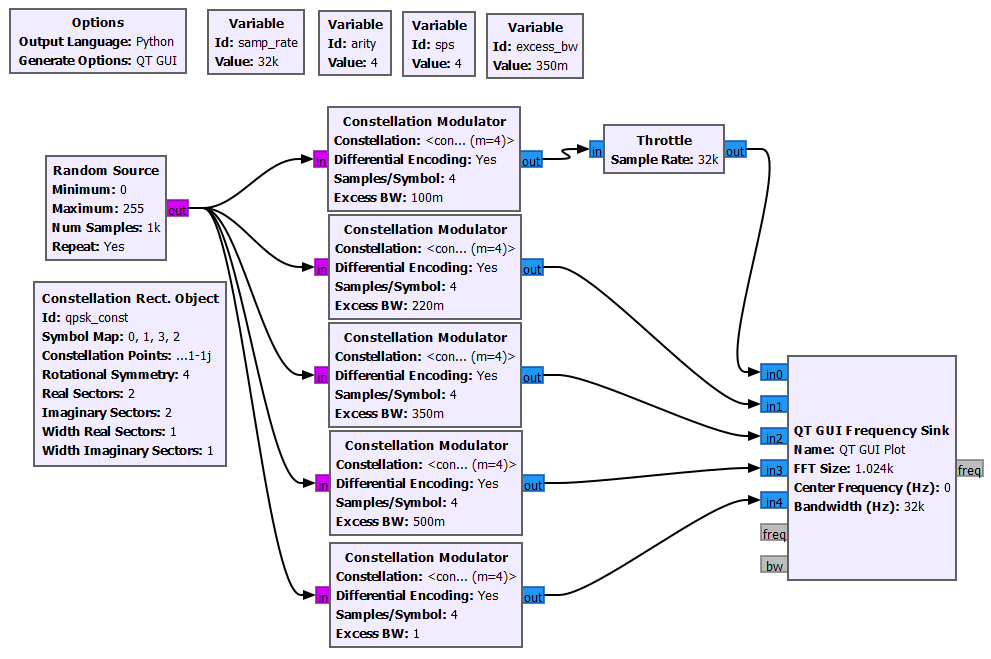
\includegraphics[width=0.8\textwidth]{fig1-1.PNG}
        \caption{Flowgraph избыточной пропускной способности}
        \label{fig:fig1-1}
\end{figure} 

    При запуске этого flowgraph, мы получаем график, показывающий различные значения избыточной пропускной способности (Рис.1.2). Типичные значения находятся в диапазоне от 0,2 (красная кривая) до 0,35 (зеленая кривая).
\begin{figure}[H]
        \centering
        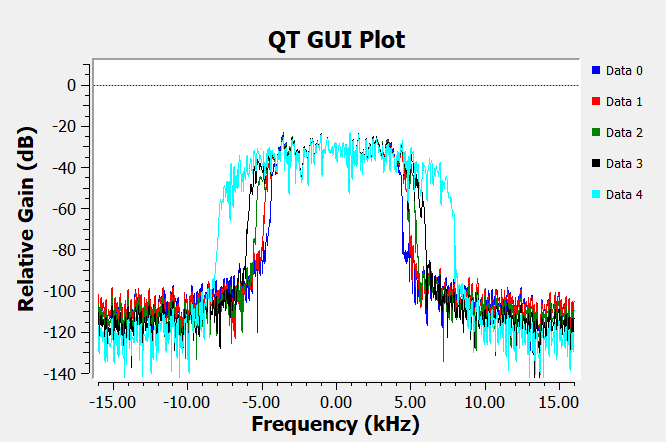
\includegraphics[width=0.8\textwidth]{fig1-2.PNG}
        \caption{Избыточная пропускная способность}
        \label{fig:fig1-2}
\end{figure}    
    
    Теперь запустим flowgraph \texttt{mpsk\_stage1.grc}, передающий созвездие QPSK (Рис.1.3).
\begin{figure}[H]
        \centering
        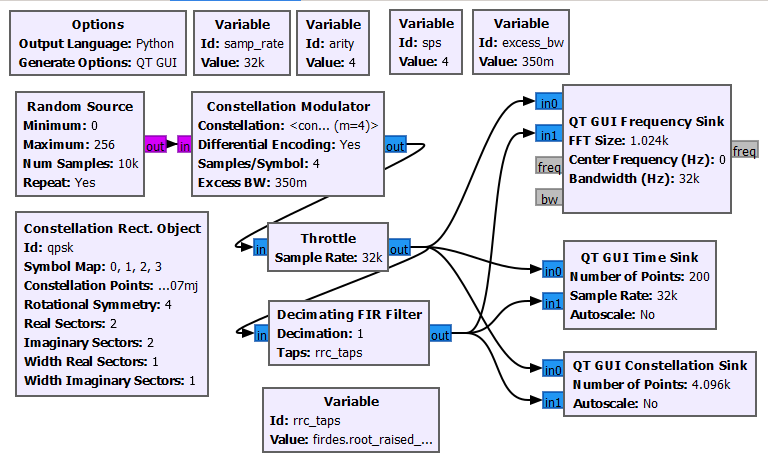
\includegraphics[width=0.8\textwidth]{fig1-3.PNG}
        \caption{Flowgraph созвездия QPSK}
        \label{fig:fig1-3}
\end{figure}
\begin{figure}[H]
        \centering
        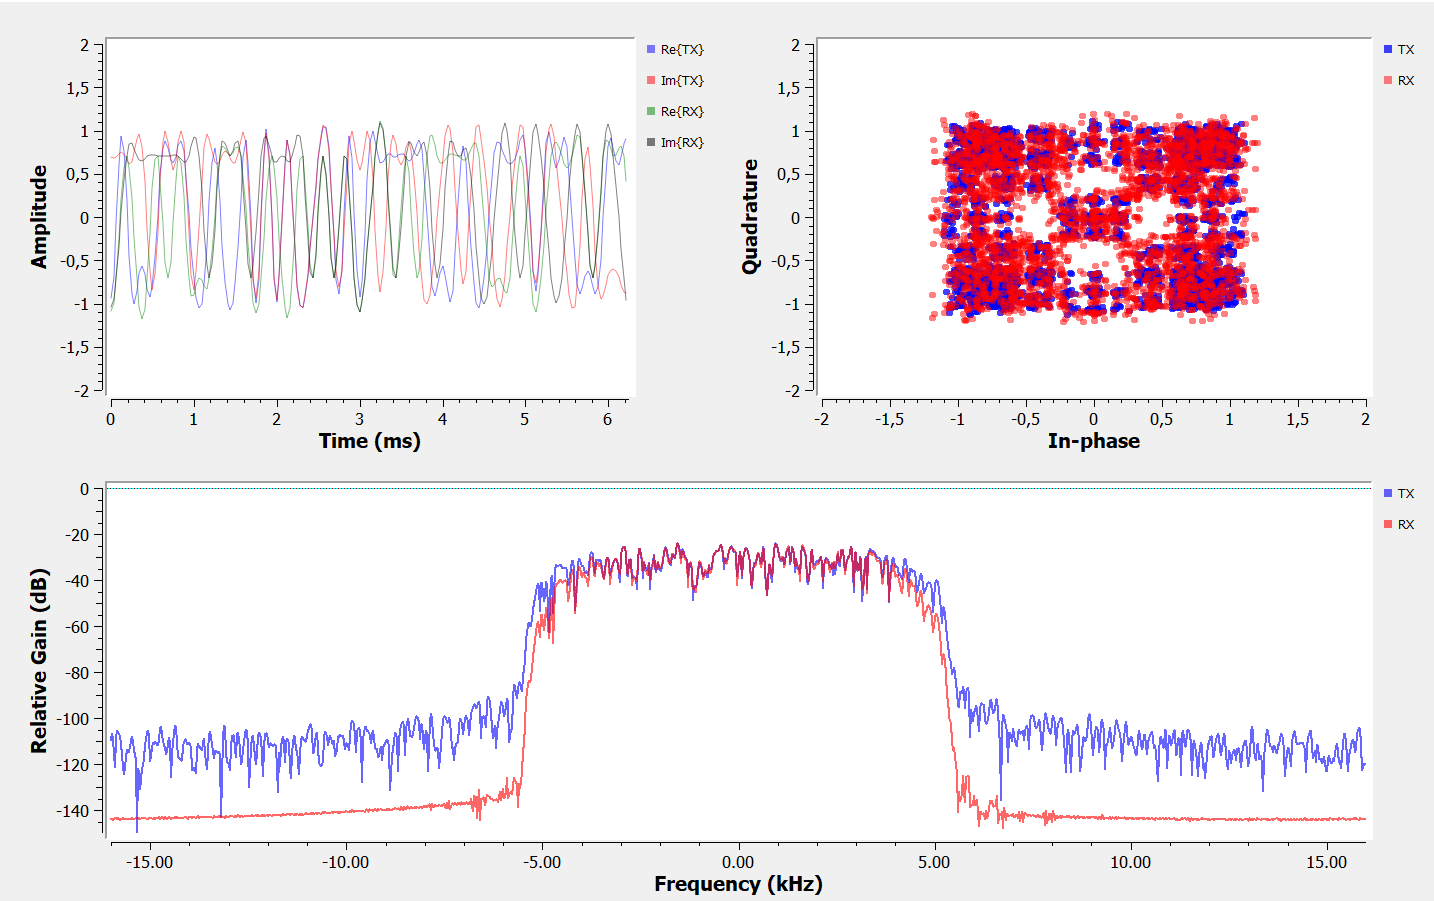
\includegraphics[width=0.8\textwidth]{fig1-4.PNG}
        \caption{Созвездие QPSK}
        \label{fig:fig1-4}
\end{figure}

    На рис.1.4 мы видим эффекты повышающей дискретизации и процесс фильтрации. 
    
    На передачике мы используем фильтр RRC, который добавляет межсимвольные помехи (ISI). На приёмнике мы используем другой фильтр RRC  для устранения ISI. Таким образом, мы сворачиваем два фильтра RRC вместе и получаем фильтр с приподнятым косинусом. 
    
    Фильтрация представляет собой свертку, поэтому выходной сигнал RRC-фильтра на приемной стороне представляет собой сигнал в форме приподнятого косинусоидального импульса с минимизированным ISI. 
    
     Получается, что на приёмнике мы используем согласованный фильтр. 
     
     Согласованный фильтр — линейный оптимальный фильтр, предназначеный для выделения сигналов известной формы на фоне шумов.

\chapter{Добавление нарушений канала}
    Теперь мы рассмотрим влияние канала на то, как сигнал искажается между передачей и приёмом. Для начала мы будем использовать самый простой блок модели канала GNU Radio, который позволит нам смоделировать несколько основных проблем связанных с приёмником.
    
    Проблемы: 
\begin{enumerate} 
  \item Шум. 
  
    В нашем приемнике вызывается аддитивный белый гауссовский шум. Мы устанавливаем мощность этого шума, регулируя значение напряжения шума модели канала.
      
  \item Часы, определяющие частоту радиомодулей.
  
    Два радиомодуля имеют разные часы. Одно радио работает на частоте \texttt{fc + f\_delta\_1}. Другое радио имеет другие часы и его реальная частота равна \texttt{fc + f\_delta\_2}. Таким образом, полученный сигнал будет \texttt{f\_delta\_1 + f\_delta\_2}.
    
  \item Идеальная точка выборки.
  
    Идеальная точка выборки связана с проблемой часов. Два радиомодуля работают с разной скоростью, поэтому идеальная точка выборки неизвестна.
\end{enumerate}

    В результате моделирования, полученный flowgraph позволяет нам поработать с аддитивным шумом, сдвигом частоты и временным сдвигом (Рис.2.1).
\begin{figure}[H]
        \centering
        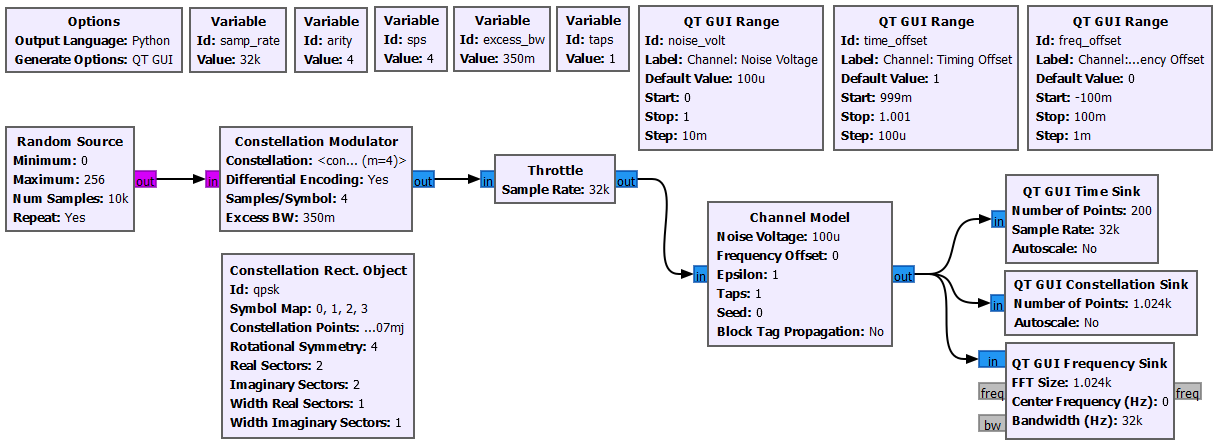
\includegraphics[width=0.8\textwidth]{fig2-1.PNG}
        \caption{Flowgraph с нарушениями канала}
        \label{fig:fig2-1}
\end{figure}
\begin{figure}[H]
        \centering
        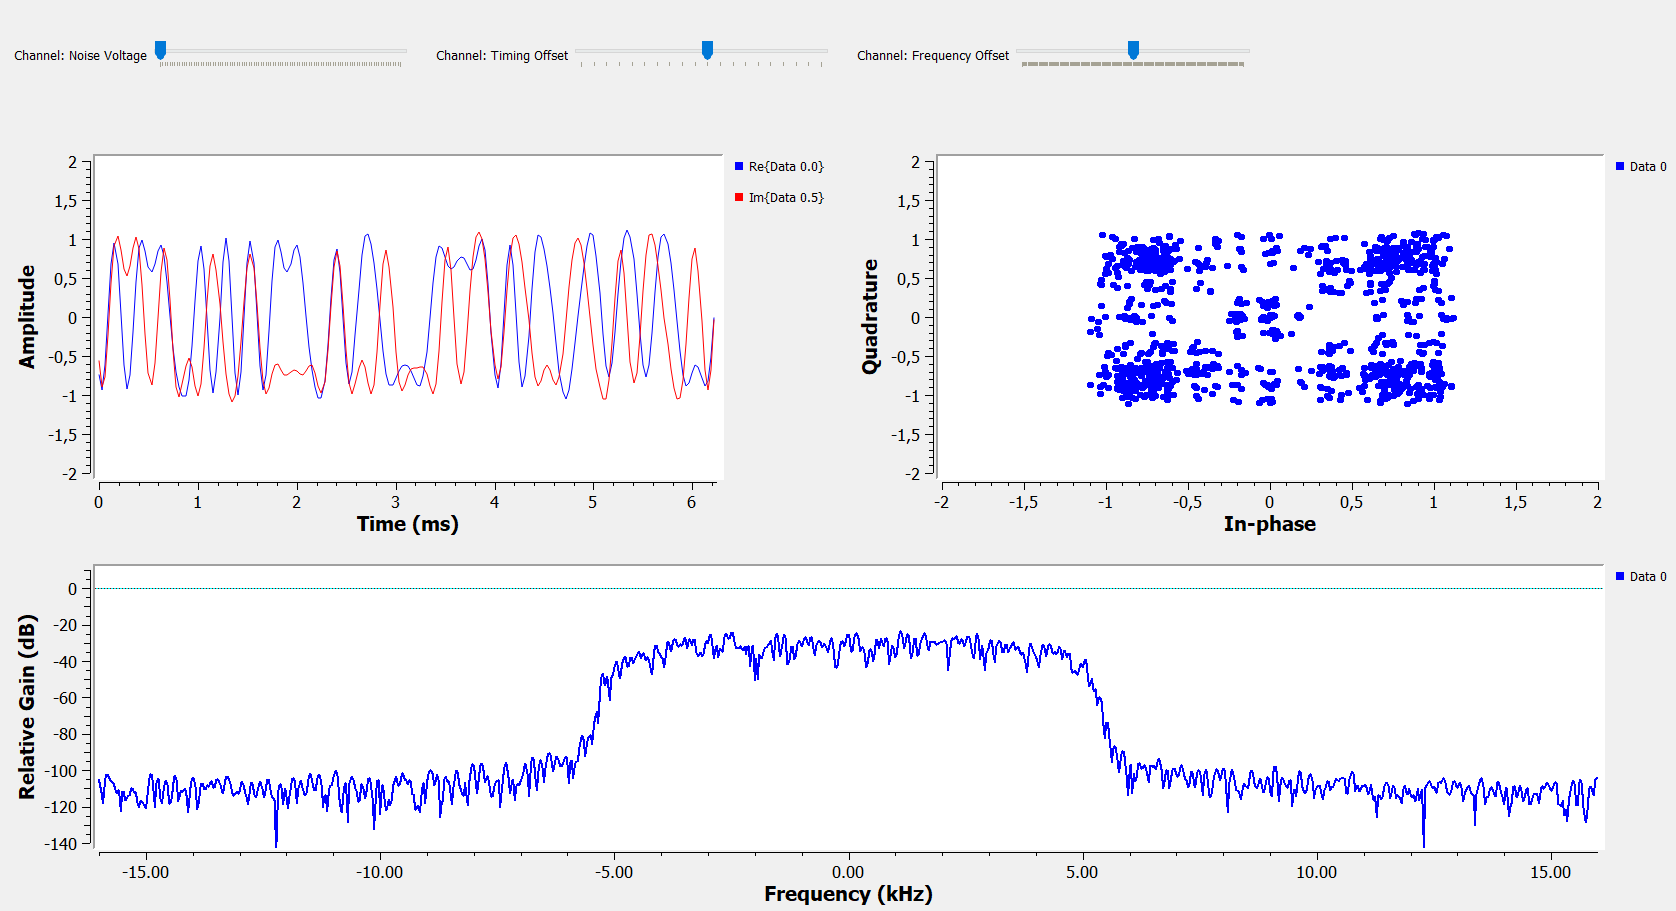
\includegraphics[width=0.8\textwidth]{fig2-2.PNG}
        \caption{Созвездие с нарушениями}
        \label{fig:fig2-2}
\end{figure}
    
    Как мы можем видеть на рис.2.2, график созвездия показывает нам облако образцов хуже, чем на предыдущем этапе. Теперь мы должны отменить все эти эффекты.

\chapter{Восстановление времени}
    Теперь перейдём к процессу восстановления. Здесь мы будем использовать алгоритм восстановления многофазных часов.
    
    Мы начнем с восстановления времени. Мы пытаемся найти наилучшее время для дискретизации входящих сигналов, что позволит максимизировать отношение сигнал/шум (SNR) каждой выборки, а также уменьшить влияние межсимвольных помех (ISI).

\section{Проблема ISI}        
    Проблему ISI мы можем увидеть на примере flowgraph \texttt{symbol\_sampling.grc}, где мы создаем четыре отдельных символа, а затем фильтруем их (Рис.3.1).
\begin{figure}[H]
        \centering
        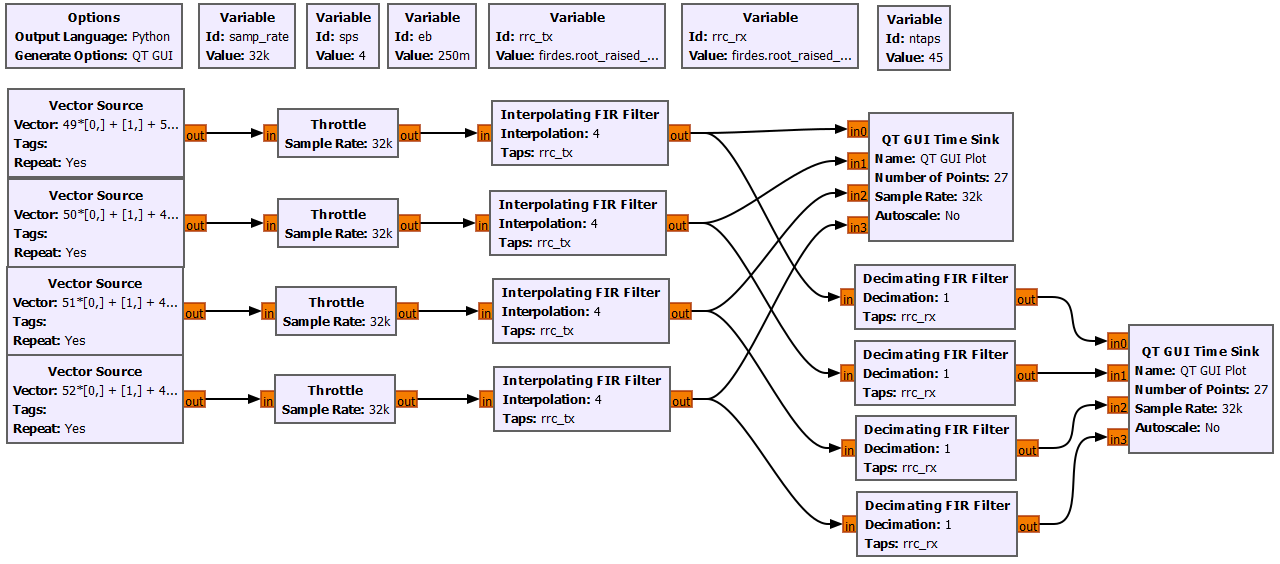
\includegraphics[width=0.8\textwidth]{fig3-1.PNG}
        \caption{Flowgraph проблемы ISI}
        \label{fig:fig3-1}
\end{figure}
\begin{figure}[H]
        \centering
        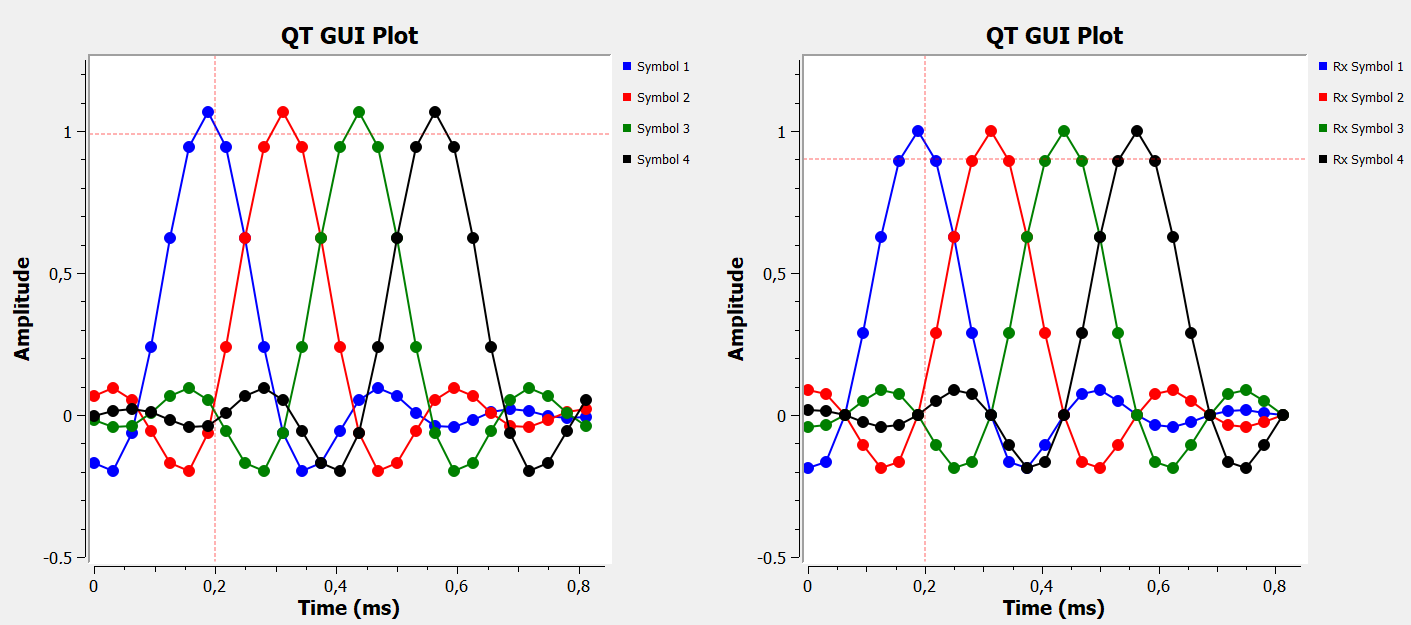
\includegraphics[width=0.8\textwidth]{fig3-2.PNG}
        \caption{Сравнение символов, отфильтрованных RC и RRC}
        \label{fig:fig3-2}
\end{figure} 

    На рис.3.2 мы видим выходные данные, которые показывают различия между символами, отфильтрованными RC и RRC. 
    
    Без фильтрации Найквиста (RRC - справа) мы можем увидеть, как в идеальной точке выборки каждого символа другие символы имеют некоторую энергию. Если мы суммируем эти символы вместе (как в непрерывном потоке), то энергия других выборок складывается вместе и искажает символ в этой точке. 
    
    И наоборот, на выходе с RC-фильтром энергия от других выборок равна 0 в идеальной точке дискретизации для данного символа во времени. Это означает, что если мы делаем выборку точно в правильной точке выборки, мы получаем энергию только от текущего символа без помех от других символов в потоке.
    
    Это моделирование позволяет нам легко настроить количество выборок на символ, избыточную полосу пропускания фильтров RRC и количество ответвлений.
    
\section{Разные часы}
    Затем мы посмотрим, как разные часы влияют на точки выборки между передатчиком и приемником. Используя пример потокового графа в \texttt{symbol\_sampling\_diff.grc}, мы моделируем влияние разных часов в передатчике и приемнике (Рис.3.3).
\begin{figure}[H]
        \centering
        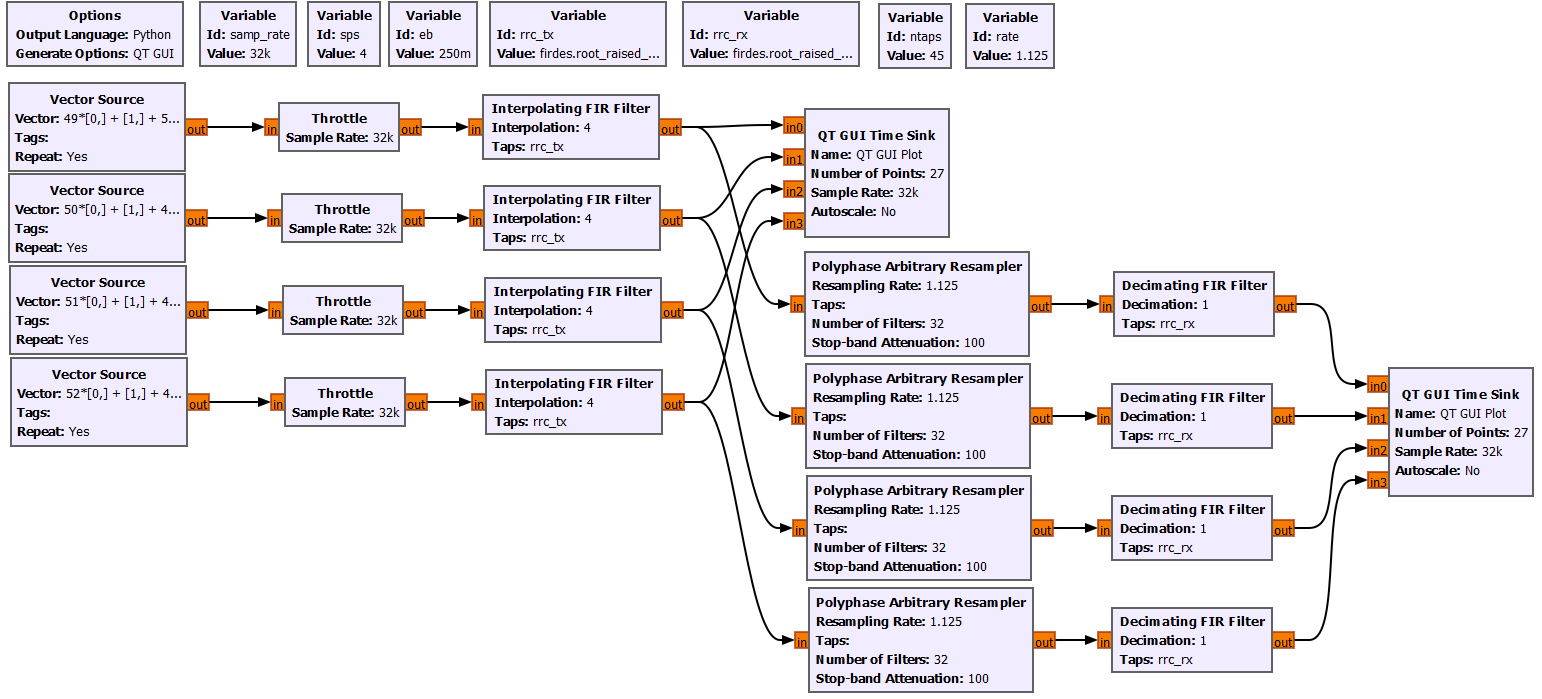
\includegraphics[width=0.8\textwidth]{fig3-3.PNG}
        \caption{Flowgraph разные часы}
        \label{fig:fig3-3}
\end{figure}
    
    Все часы несовершенные, поэтому они (Рис.3.4):
\begin{enumerate} 
  \item начнут свою работу в разные моменты времени; 
  \item дрейфуют относительно других часов.
\end{enumerate}
\begin{figure}[H]
        \centering
        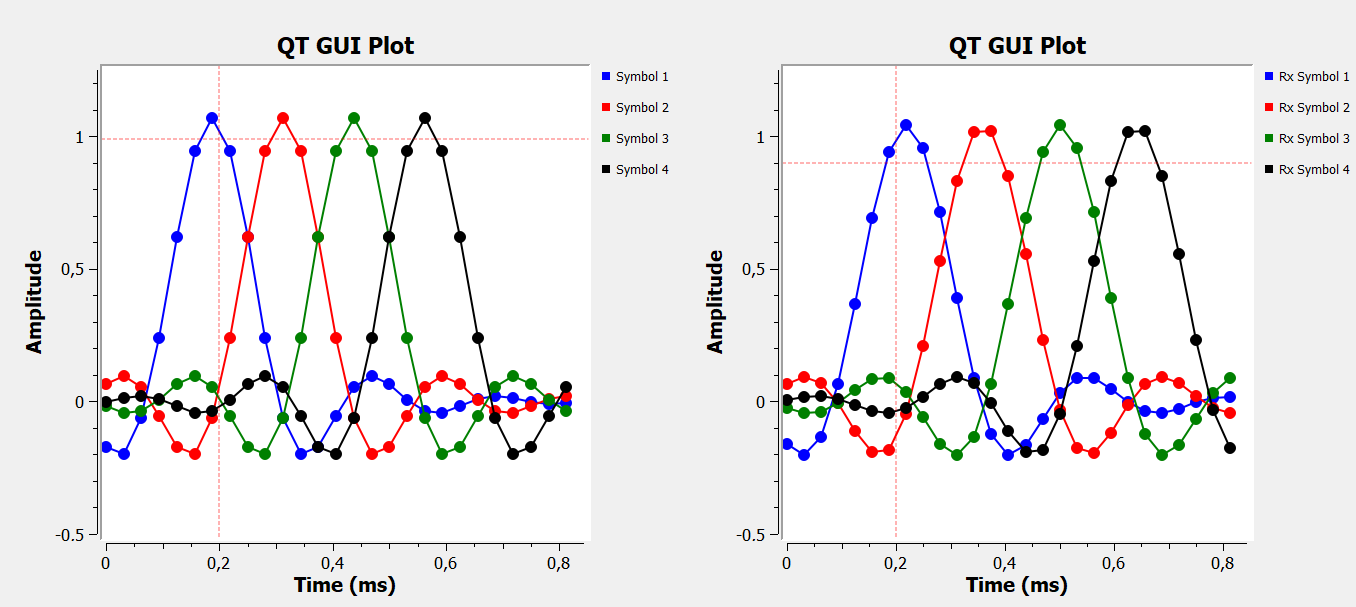
\includegraphics[width=0.8\textwidth]{fig3-4.PNG}
        \caption{Работа разных часов}
        \label{fig:fig3-4}
\end{figure}

    Наша задача - синхронизировать часы передачи и приемника, используя только информацию в приемнике из входящих выборок. Это задача известна как восстановление часов или времени.
    
\section{Блок синхронизации многофазных часов}
    Изучим как работает блок синхронизации многофазных часов перед его применением.
    
\subsection{Один фильтр}        
    Блок вычисляет первый дифференциал входящего сигнала, который будет связан с его смещением тактовой частоты. Используя пример flowgraph \texttt{symbol\_differential\_filter.grc} (Рис.3.5), мы можем увидеть графики с параметром скорости 1 (т.е. нет смещения часов).
    
    Очевидно, что нам нужен образец 0,22 мс. Фильтр разности ([-1, 0, 1]) генерирует дифференциал символа, и, как показано на рис.3.6, выходной сигнал этого фильтра в правильной точке выборки равен 0. Затем мы можем инвертировать этот оператор и вместо этого сказать, когда выход дифференциального фильтра равен 0, мы нашли оптимальную точку выборки.
\begin{figure}[H]
        \centering
        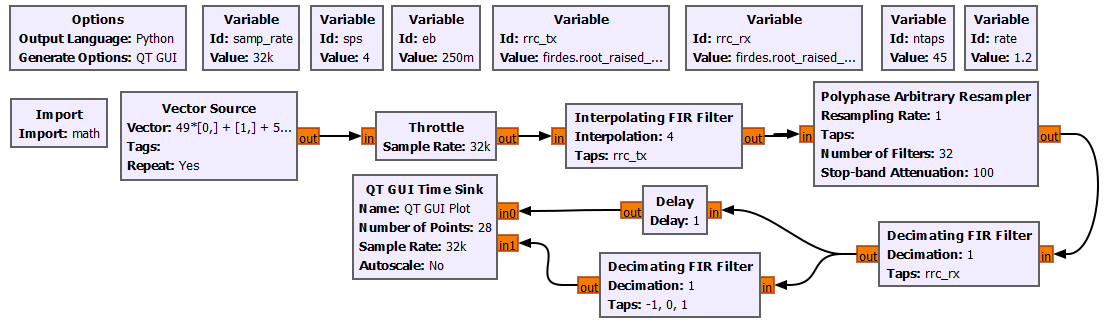
\includegraphics[width=0.8\textwidth]{fig3-5.PNG}
        \caption{Flowgraph с использованием блока}
        \label{fig:fig3-5}
\end{figure}
\begin{figure}[H]
        \centering
        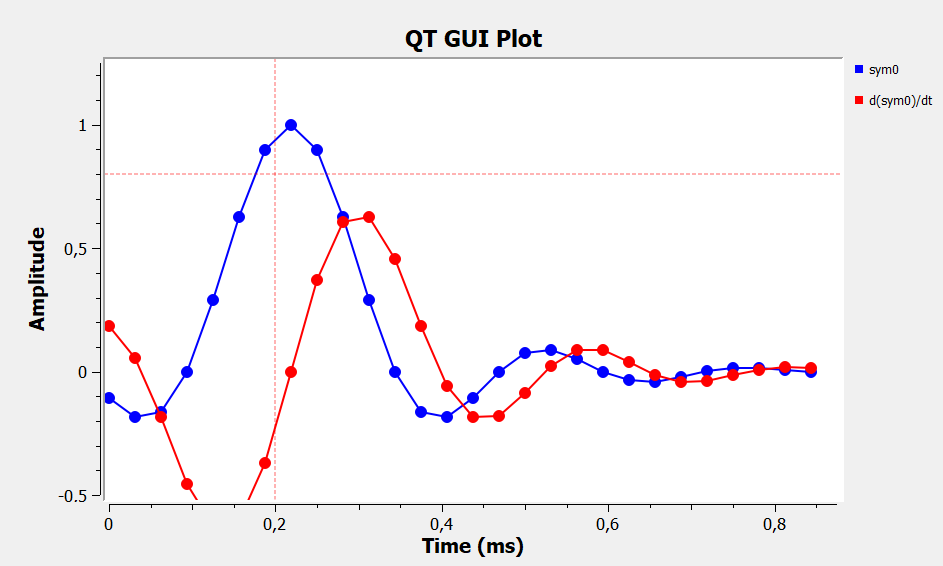
\includegraphics[width=0.8\textwidth]{fig3-6.PNG}
        \caption{Нет смещения часов}
        \label{fig:fig3-6}
\end{figure}
    
    У нас есть временное смещение там, где пик символа выключен, а производный фильтр не показывает нам нулевую точку (Рис.3.7).
\begin{figure}[H]
        \centering
        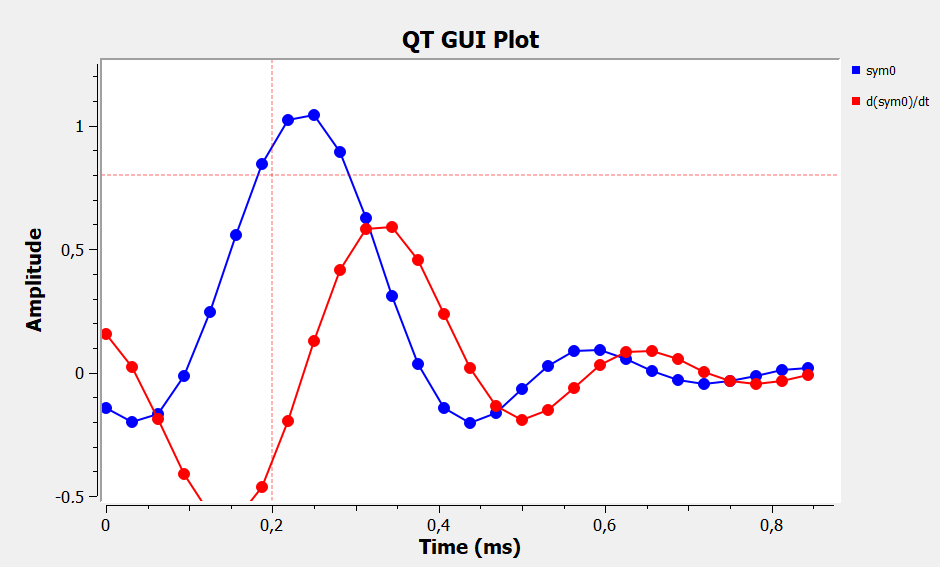
\includegraphics[width=0.8\textwidth]{fig3-7.PNG}
        \caption{Есть смещение часов}
        \label{fig:fig3-7}
\end{figure}

\subsection{Несколько фильтров} 
    Вместо использования одного фильтра мы можем создать серию фильтров, каждый с разной фазой. Если у нас достаточно фильтров на разных фазах, один из них имеет правильную фазу фильтра, которая даст нам желаемое значение синхронизации. Посмотрим на симуляцию, которая строит 5 фильтров, что означает 5 различных фаз (Рис.3.8).
\begin{figure}[H]
        \centering
        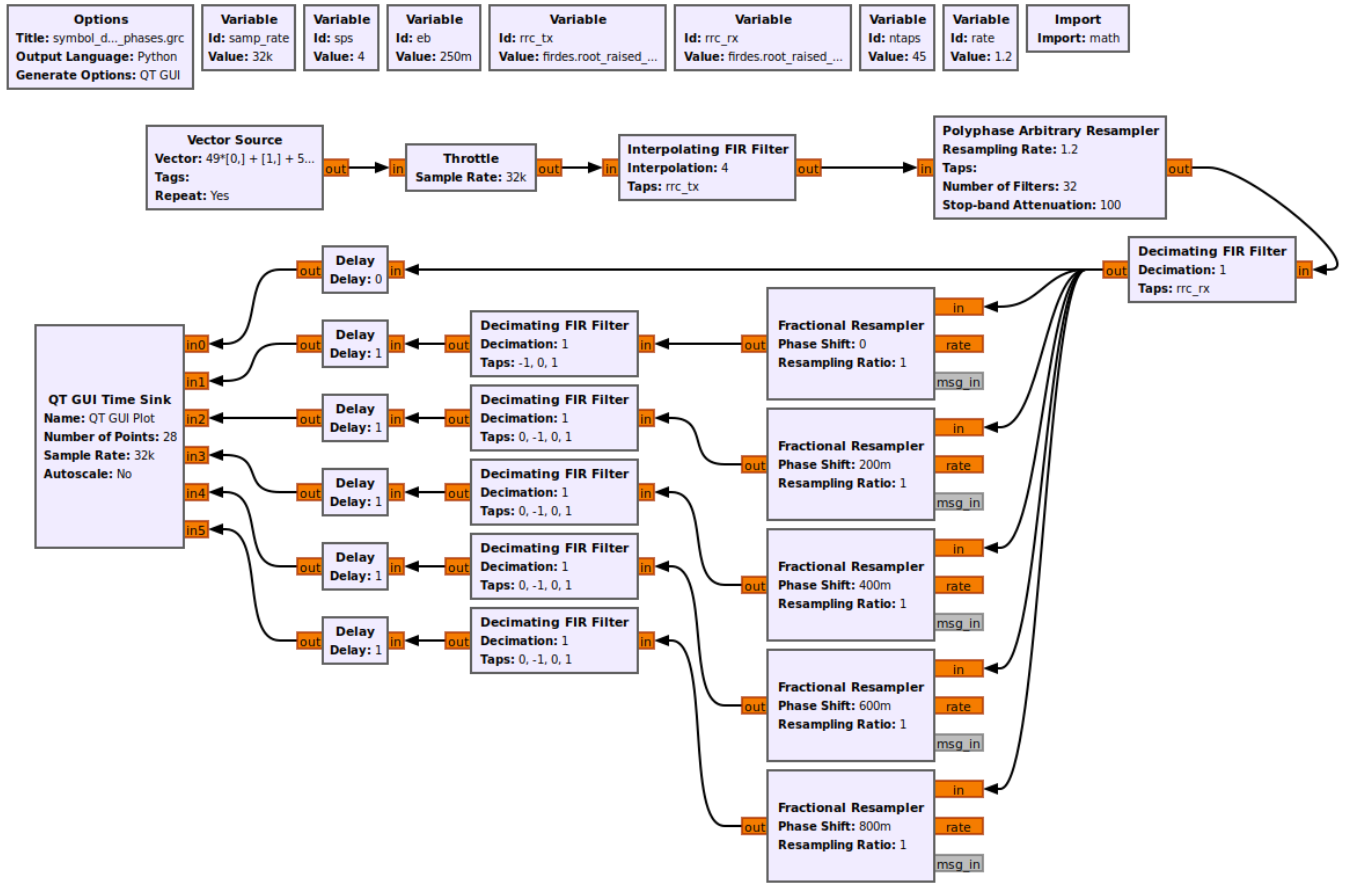
\includegraphics[width=0.8\textwidth]{fig3-8.PNG}
        \caption{Flowgraph с несколькими фазами}
        \label{fig:fig3-8}
\end{figure}
\begin{figure}[H]
        \centering
        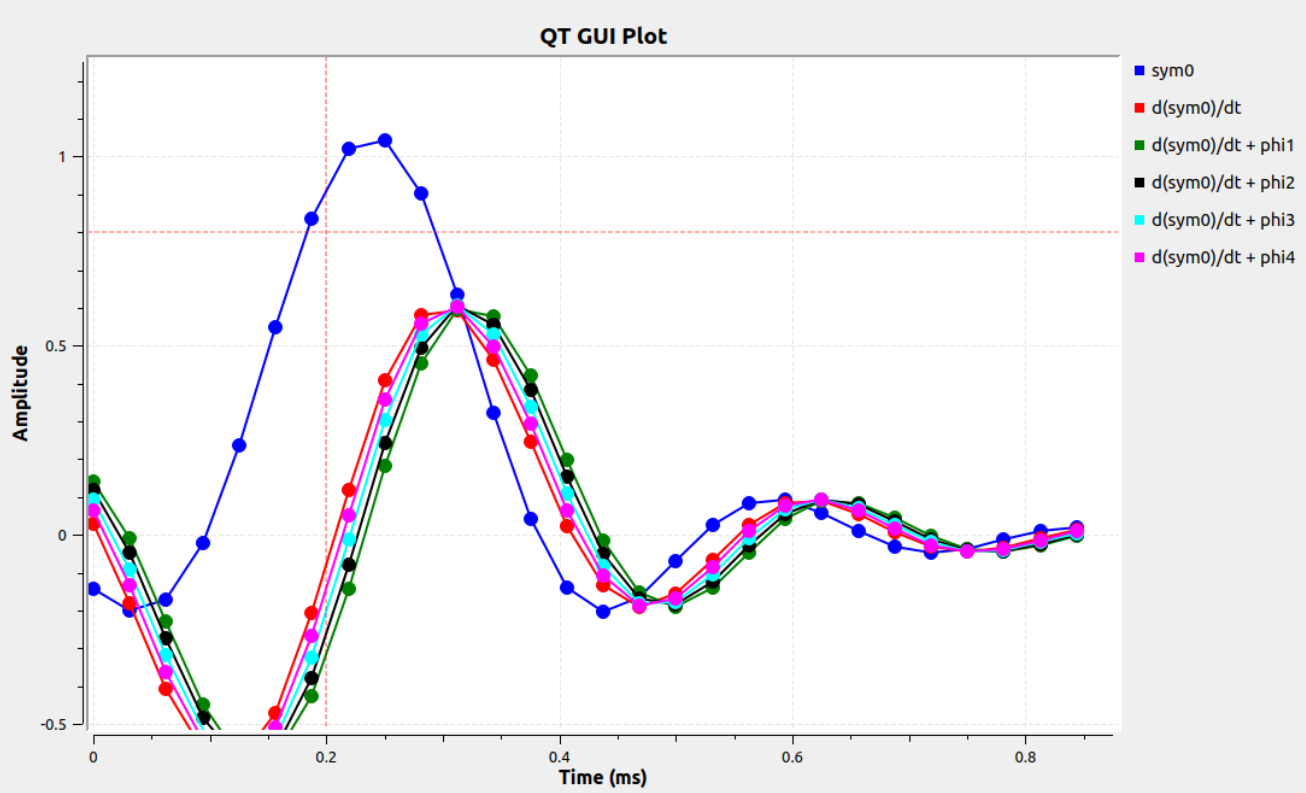
\includegraphics[width=0.8\textwidth]{fig3-9.PNG}
        \caption{Несколько фаз}
        \label{fig:fig3-9}
\end{figure} 
   
    На рис.3.9 мы можем видеть, что сигнал, помеченный как $d(sym0)/dt+phi3$, имеет точку отсчета в 0. Это говорит нам о том, что наша идеальная точка дискретизации находится при этом фазовом сдвиге. Следовательно, если мы возьмем RRC-фильтр нашего приемника и настроим его фазу на $phi3=3*2\pi/5$, то мы сможем исправить рассогласование по времени и выбрать идеальную точку дискретизации.
    
    Итак, в данном примере мы использовали 5 фильтров в качестве идеальной точки выборки. Но этого недостаточно. Любое смещение выборки между этими фазами по-прежнему приведет к несвоевременной выборке с добавленными ISI, как мы исследовали ранее.
    
    Поэтому мы используем больше фильтров (32), чтобы получить максимальный коэффициент шума ISI, который меньше шума квантования 16-битного значения. То есть мы получим точность 16 бит. Для большей точность потребуется больше фильтров.
    
    Затем мы используем контур управления 2-го порядка, который требуется, чтобы получить как правильную фазу фильтра, так и разницу в скорости между двумя тактовыми сигналами.
    
\section{Использование блока многофазной синхронизации}
    Теперь мы используем этот блок в нашей симуляции. Пример flowgraph \texttt{mpsk\_stage3.grc} принимает выходные данные модели канала и передает их через наш блок (Рис.3.10).
\begin{figure}[H]
        \centering
        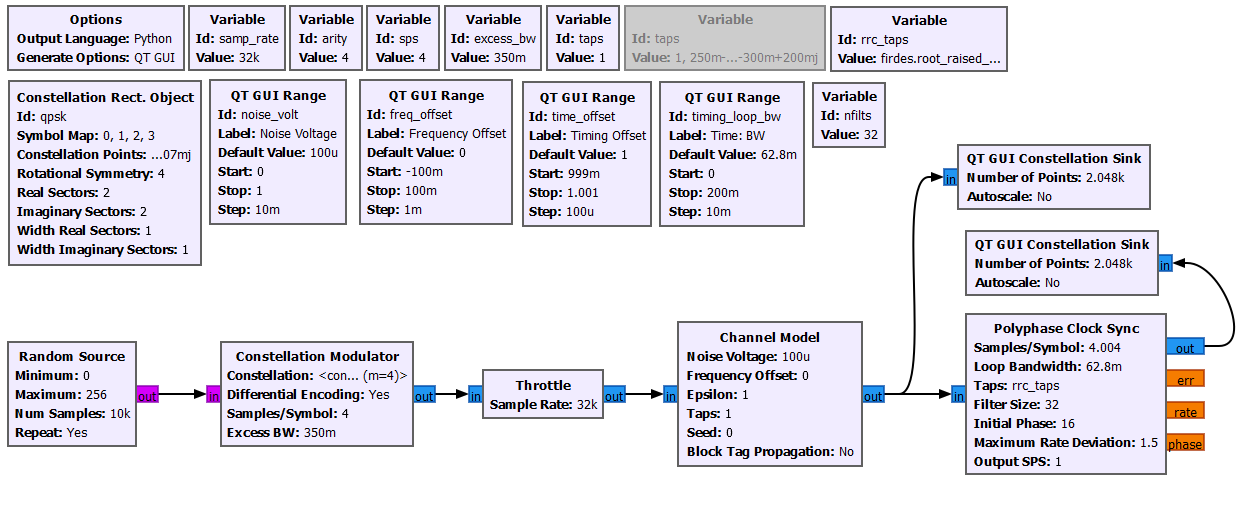
\includegraphics[width=0.8\textwidth]{fig3-10.PNG}
        \caption{Flowgraph с блоком многофазной синхронизации}
        \label{fig:fig3-10}
\end{figure}
\begin{figure}[H]
        \centering
        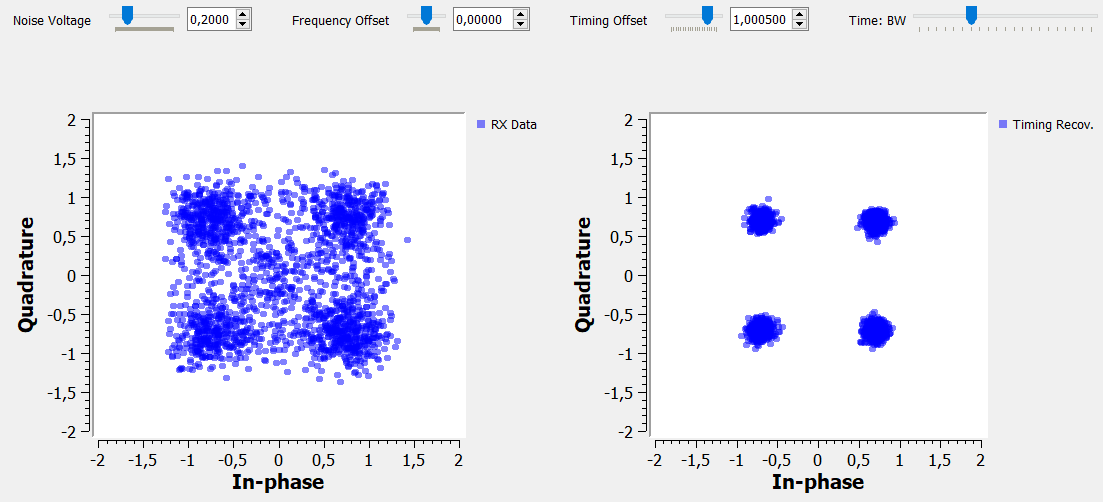
\includegraphics[width=0.8\textwidth]{fig3-11.PNG}
        \caption{Использование блока многофазной синхронизации}
        \label{fig:fig3-11}
\end{figure}

    На рис.3.11 мы видим два созвездия: слева - полученный сигнал до восстановления синхронизации и справа - после восстановления синхронизации. 
    
    Мы можем изменять разные параметны  наблюдать за изменением созвездия. Например, когда мы добавляем частотный сдвиг, мы видим, что созвездие становится кругом (Рис.3.12).
\begin{figure}[H]
        \centering
        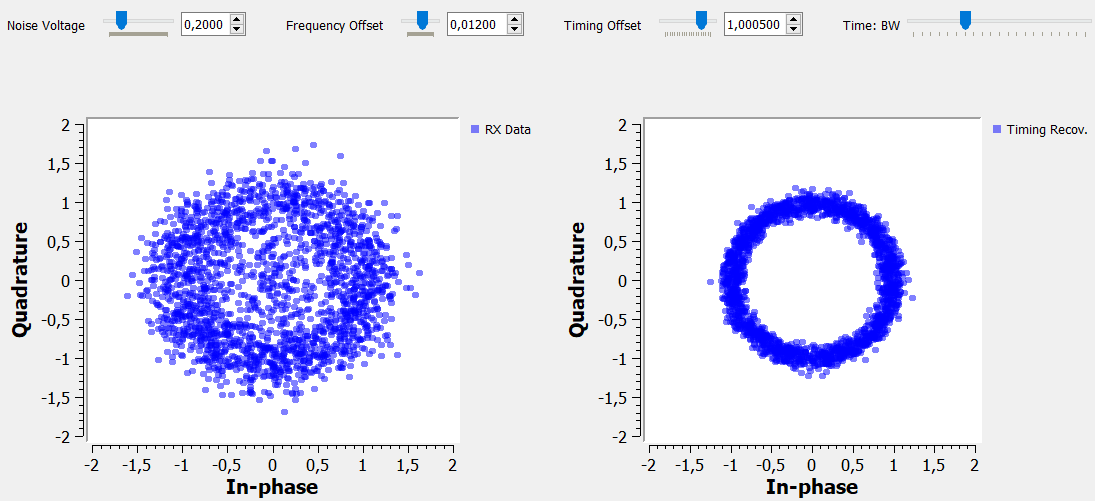
\includegraphics[width=0.8\textwidth]{fig3-12.PNG}
        \caption{Добавление частотного сдвига}
        \label{fig:fig3-12}
\end{figure}

\chapter{Многолучевость}
    Сначала мы разберемся, что такое многолучевость. В большинстве коммуникационных сред у нас нет единственного пути для прохождения сигнала от передатчика к приемнику. Сигналы отражаются от различных поверхностей и приходят на приёмник в разное время в зависимости от длины пути. Их суммирование в приемнике вызывает искажения. Эти искажения вызывают внутрисимвольную и межсимвольную интерференции. 
    
    Нам нужно исправить это поведение, и мы можем сделать это, используя механизм, очень похожий на стереоэквалайзер. С помощью стереофонического эквалайзера мы можем изменить усиление определенных частот, чтобы либо подавить, либо усилить эти сигналы (Рис.4.1). 
\begin{figure}[H]
        \centering
        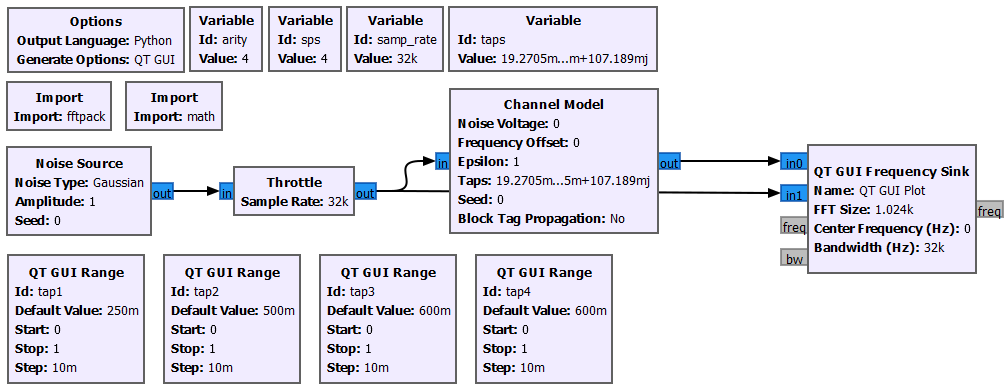
\includegraphics[width=0.8\textwidth]{fig4-1.PNG}
        \caption{Flowgraph многолучевость}
        \label{fig:fig4-1}
\end{figure}
\begin{figure}[H]
        \centering
        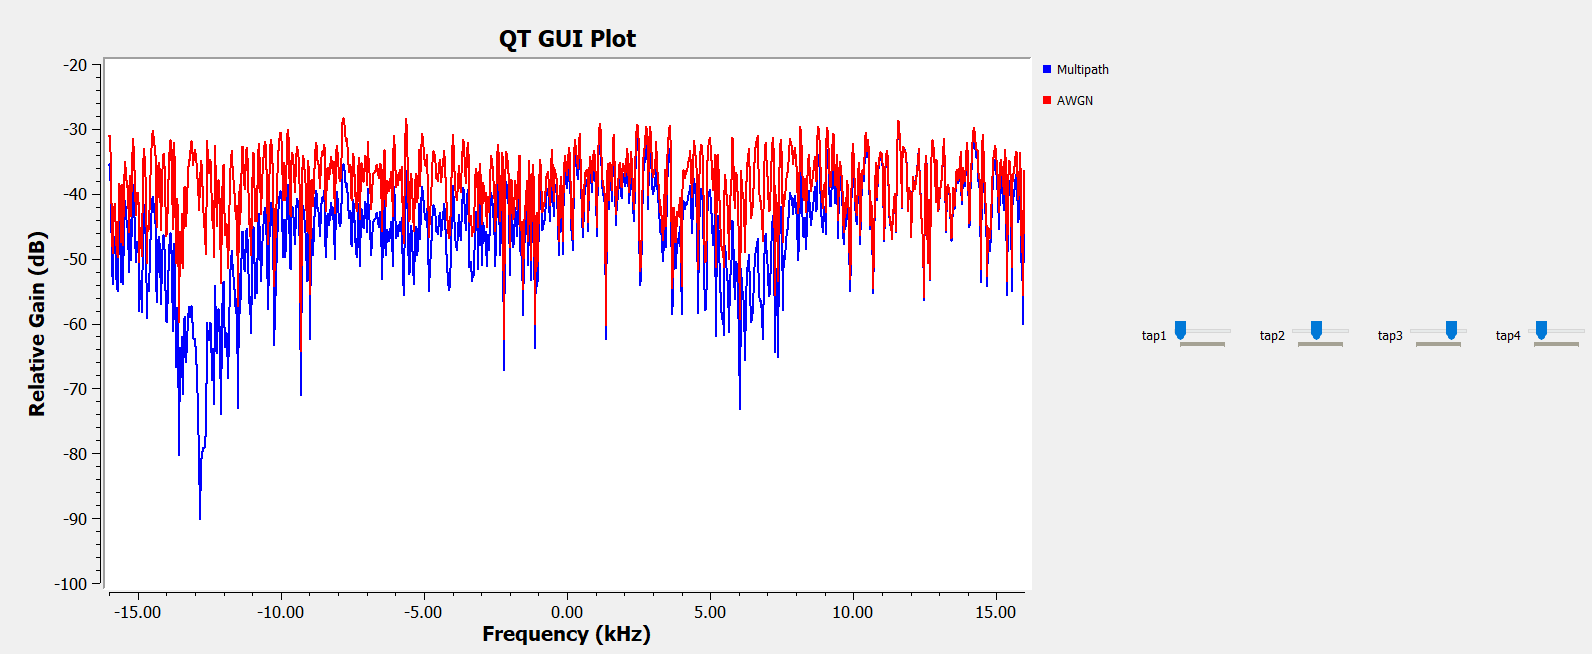
\includegraphics[width=0.8\textwidth]{fig4-2.PNG}
        \caption{Использование блока многофазной синхронизации}
        \label{fig:fig4-2}
\end{figure}    
    
    Как мы можем видеть на рис.4.2, многолучевой канал создает некоторые искажения в сигнале. Задача эквалайзера - отменить искажение, вызванное каналом, чтобы выходной сигнал эквалайзера был ровным. Но вместо того, чтобы настраивать каждый tap вручную, мы используем алгоритмы, которые обновляют эти taps за нас. Наша задача - использовать правильный алгоритм эквалайзера и настроить параметры. 
    
    Одним из важных параметров здесь является количество taps в эквалайзере. Как мы видим в нашем моделировании, пять taps дают довольно грубый контроль над частотной характеристикой. Чем больше taps, тем больше времени требуется как на вычисление ответвлений, так и на запуск эквалайзера против сигнала.
    
\chapter{Эквалайзеры}
    GNU Radio имеет два эквалайзера.
\section{Эквалайзер CMA}
    CMA или алгоритм постоянного модуля - это слепой эквалайзер, который работает только с сигналами с постоянной амплитудой или модулем.
    
    В примере \texttt{mpsk\_stage4.grc} мы используем алгоритм CMA с 11 taps (Рис.5.1). Изменим параметры и посмотрим, как это влияет на производительность как с точки зрения вычислений, так и с точки зрения сигналов.
\begin{figure}[H]
        \centering
        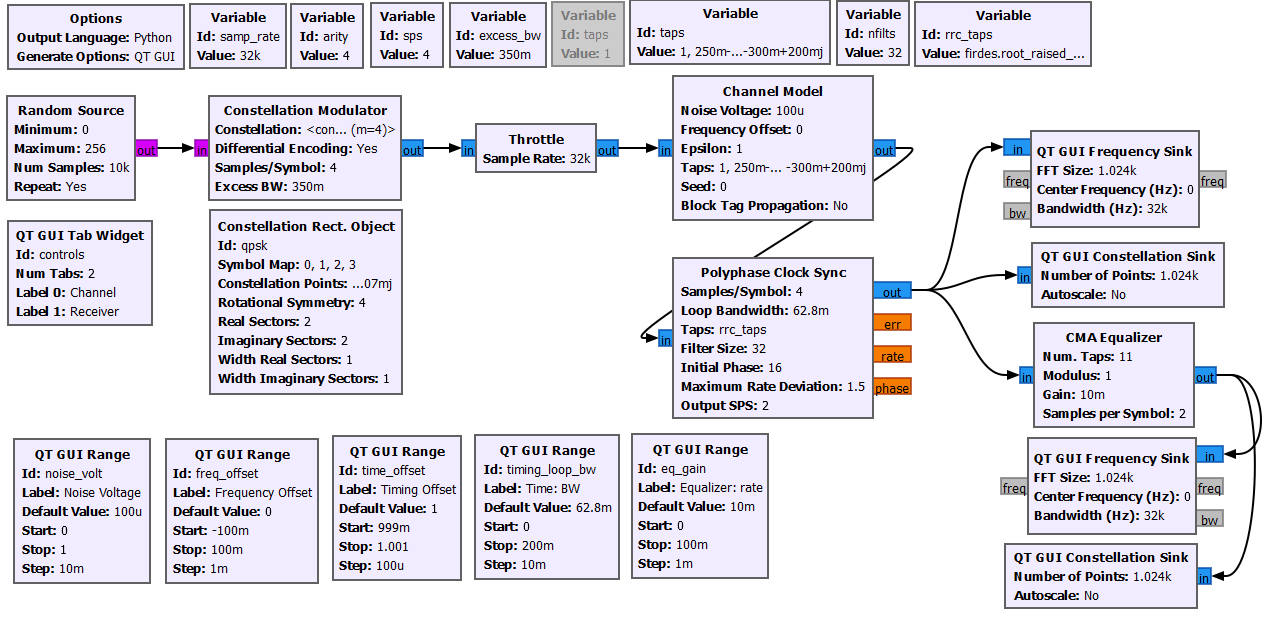
\includegraphics[width=0.8\textwidth]{fig5-1.PNG}
        \caption{Flowgraph с эквалайзером CMA}
        \label{fig:fig5-1}
\end{figure}
\begin{figure}[H]
        \centering
        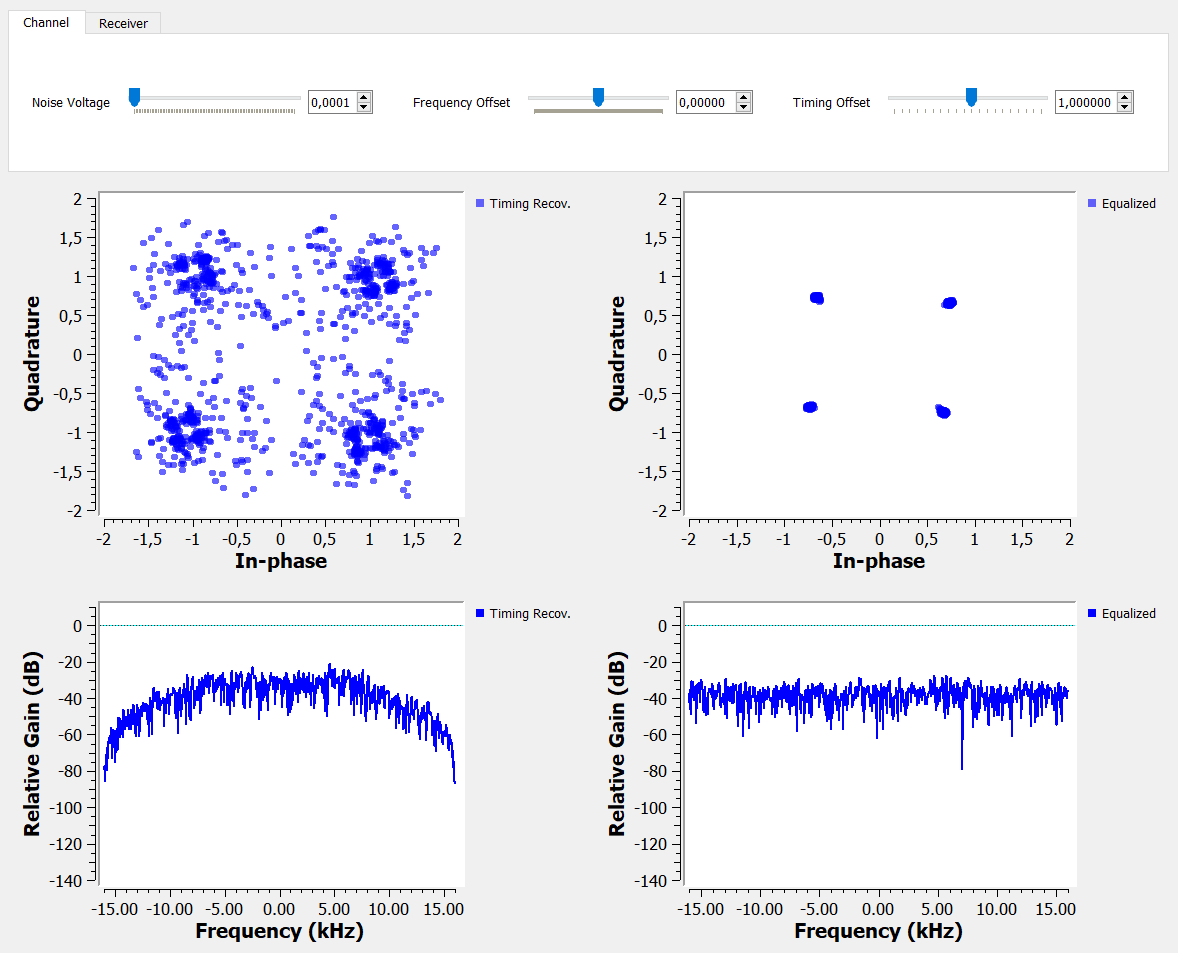
\includegraphics[width=0.8\textwidth]{fig5-2.PNG}
        \caption{Использование эквалайзера CMA}
        \label{fig:fig5-2}
\end{figure}    
        
    На рис.5.2 мы можем увидеть эффект синхронизированного по времени многолучевого сигнала до и после эквалайзера. До эквалайзера у нас очень некрасивый сигнал даже без шумов. Эквалайзер понимает, как инвертировать и сократить канал, чтобы у нас снова был хороший, чистый сигнал. Мы также можем видеть сам канал и то, как он красиво выравнивается после эквалайзера. 
\section{Эквалайзер LMS DD}
    Хорошей практикой является использование блока эквалайзера LMS DD. 
    
    LMS или алгоритм наименьших квадратов требует знания принимаемого сигнала. Эквалайзеру необходимо знать точки созвездия для корректировки, и он использует решения о выборках, чтобы сообщить, как обновлять ответвления для эквалайзера.
    
    Заменим эквалайзер CMA на LMS DD (Рис.5.3).
\begin{figure}[H]
        \centering
        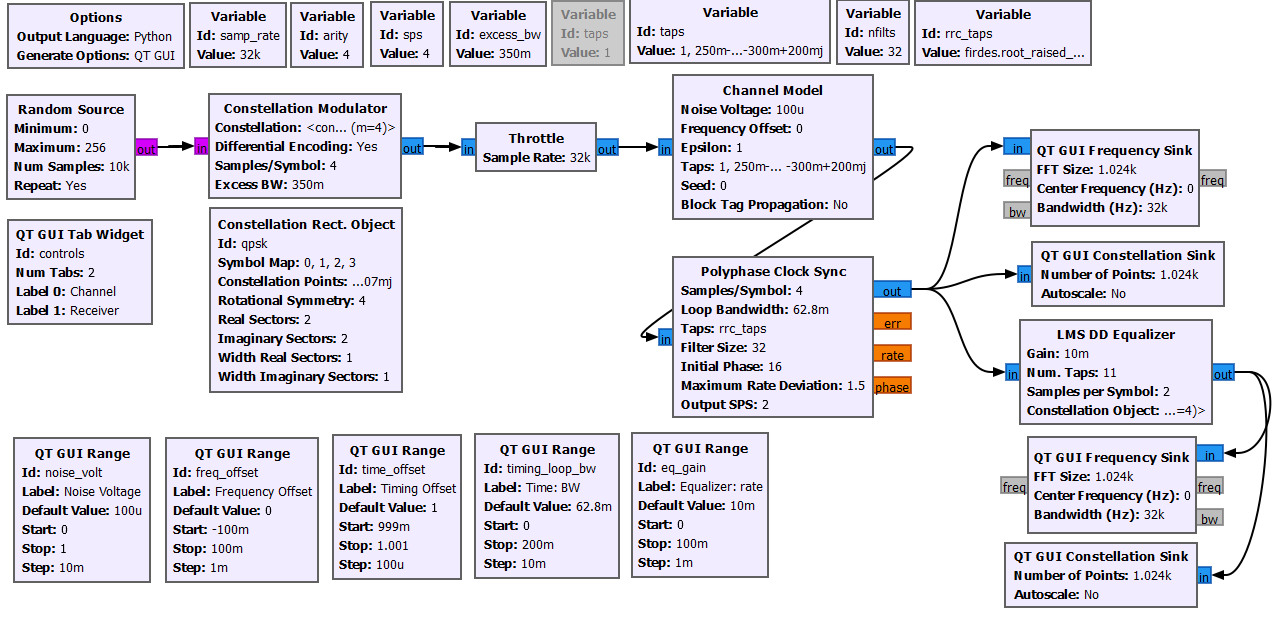
\includegraphics[width=0.8\textwidth]{fig5-3.PNG}
        \caption{Flowgraph с эквалайзером LMS DD}
        \label{fig:fig5-3}
\end{figure}
\begin{figure}[H]
        \centering
        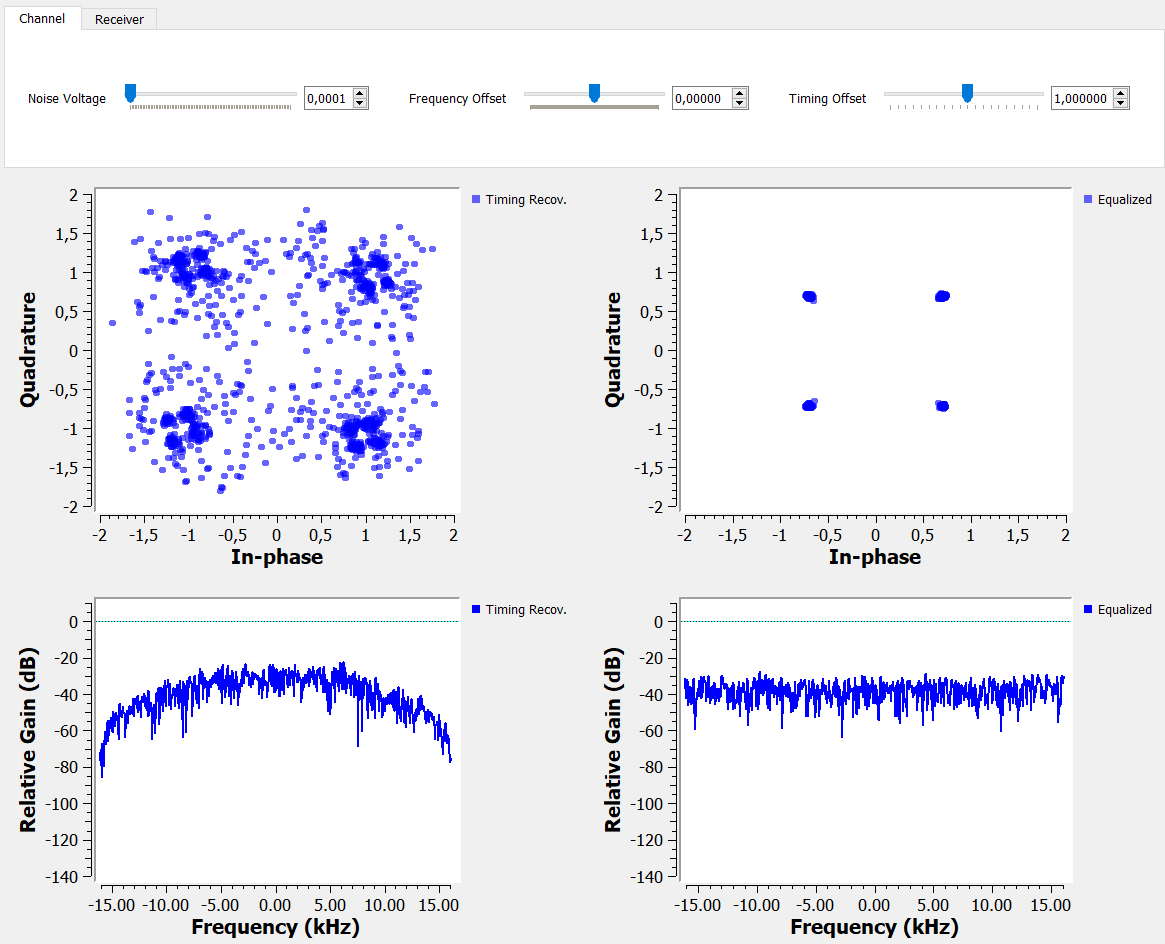
\includegraphics[width=0.8\textwidth]{fig5-4.PNG}
        \caption{Использование эквалайзера LMS DD}
        \label{fig:fig5-4}
\end{figure}

    Результат работы этого эквалайзера мы можем видеть на рис.5.4.
    
\chapter{Фазовая и точная частотная коррекция}
    Мы выровняли канал, но у нас все еще есть проблема смещения фазы и частоты. Она выходит за пределами возможностей эквалайзера. Поэтому нам нужно исправить любой сдвиг фазы, а также любой сдвиг частоты.
    
    На этом этапе мы будем использовать цикл второго порядка, чтобы мы могли отслеживать фазу и частоту. Тип восстановления, который мы здесь рассмотрим, предполагает, что мы выполняем точную частотную коррекцию. Поэтому мы должны находиться в приличном диапазоне идеальной частоты, чтобы цикл сошёлся.
    
    Для этой задачи мы собираемся использовать цикл Костаса в примере \texttt{mpsk\_stage5.grc} (Рис.6.1).
\begin{figure}[H]
        \centering
        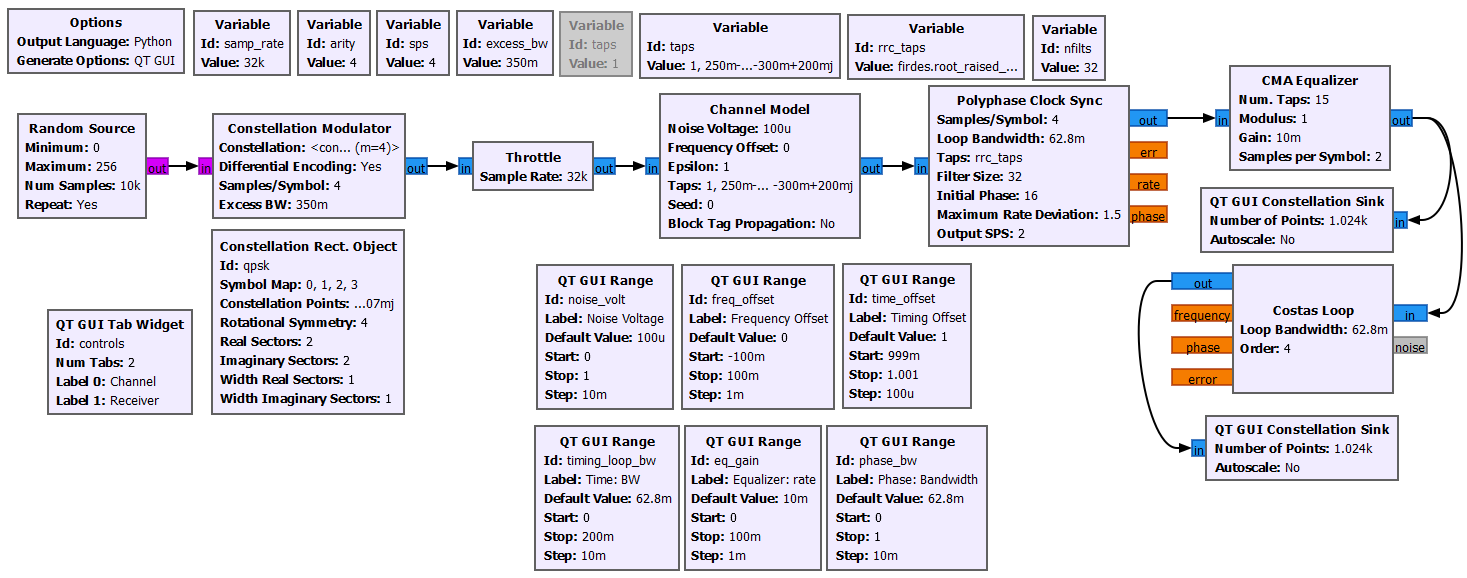
\includegraphics[width=0.8\textwidth]{fig6-1.PNG}
        \caption{Flowgraph для исправдения сдвига фазы и частоты}
        \label{fig:fig6-1}
\end{figure}
\begin{figure}[H]
        \centering
        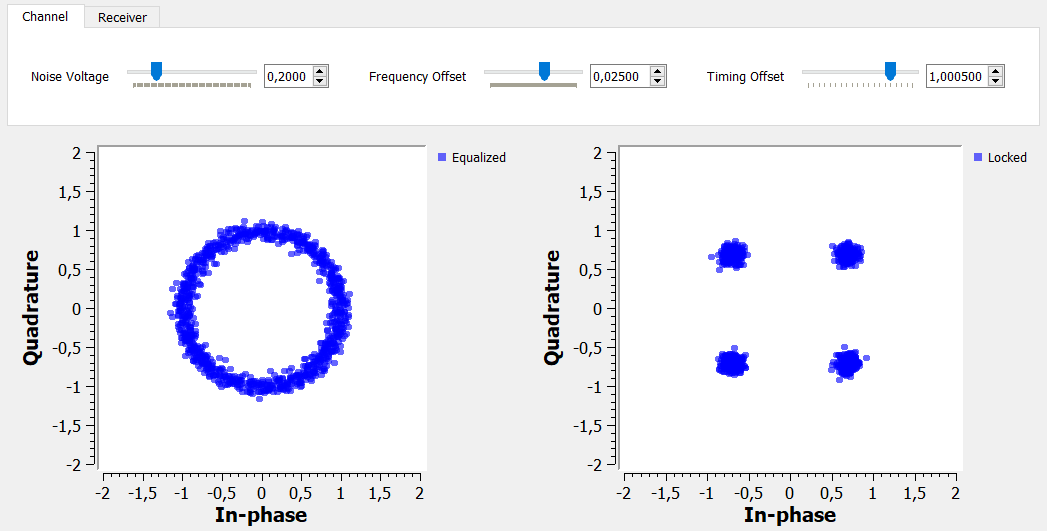
\includegraphics[width=0.8\textwidth]{fig6-2.PNG}
        \caption{Исправление сдивига фазы и частоты}
        \label{fig:fig6-2}
\end{figure}  

    На рис.6.2 мы установили шум, временной сдвиг, простой многолучевой канал и частотный сдвиг. После эквалайзера мы видим, что все символы находятся на единичном круге, но вращаются из-за смещения частоты, которое еще не исправлено. На выходе блока цикла Костаса мы можем видеть заблокированное созвездие и дополнительный шум.

\chapter{Расшифровка}
    Теперь мы можем декодировать сигнал. Используя пример flowgraph \texttt{mpsk\_stage6.grc} (Рис.7.1), мы вставляем \texttt{Constellation Decoder} после цикла Костаса, но наша работа еще не завершена. Мы передаём 4 дифференциальных символа, но мы не можем быть уверены, что у нас есть такое же отображение символов на точки созвездия, которое мы делали при передаче. 
\begin{figure}[H]
        \centering
        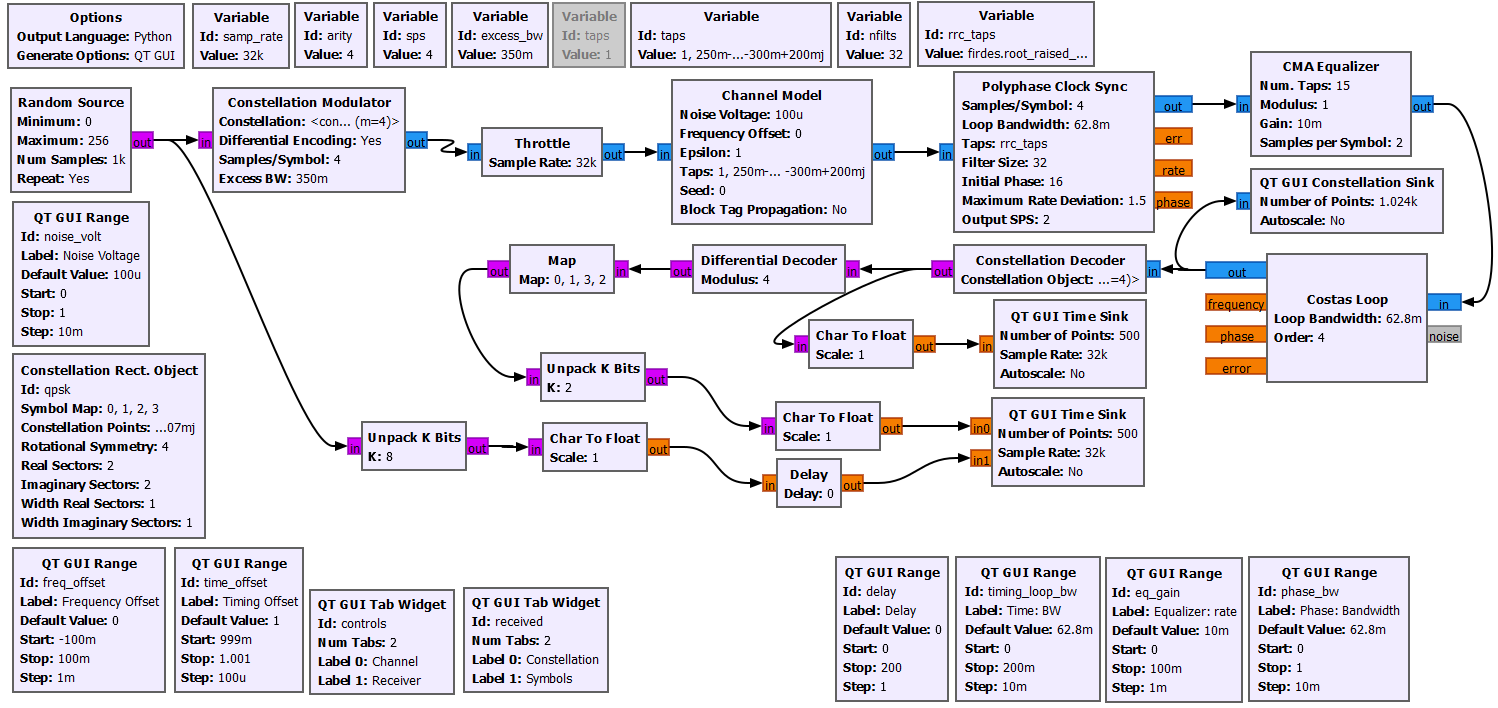
\includegraphics[width=0.8\textwidth]{fig7-1.PNG}
        \caption{Flowgraph декодирования}
        \label{fig:fig7-1}
\end{figure}
    
    Flowgraph использует блок дифференциального декодера для преобразования кодированных дифференциальным кодом символов обратно в их исходные символы. Мы используем блок Map для преобразования символов из дифференциального декодера в исходные символы, которые мы передали. На данный момент у нас теперь есть исходные символы от 0 до 3, поэтому мы распакуем эти 2 бита на символ в биты, используя блок unpack bits. Теперь у нас есть исходный битовый поток данных.
    
     Но как мы узнаем, что это исходный битовый поток? Для этого нам нужно сравнить переданные данные с входным битовым потоком. Однако прямое сравнение ничего не даст. Так как в цепочке приемника много блоков и фильтров, которые задерживают сигнал, принятый сигнал отстает на некоторое количество бит. Чтобы это исправить, необходимо добавить задержку \texttt{Delay} (Рис.7.2).
\begin{figure}[H]
        \centering
        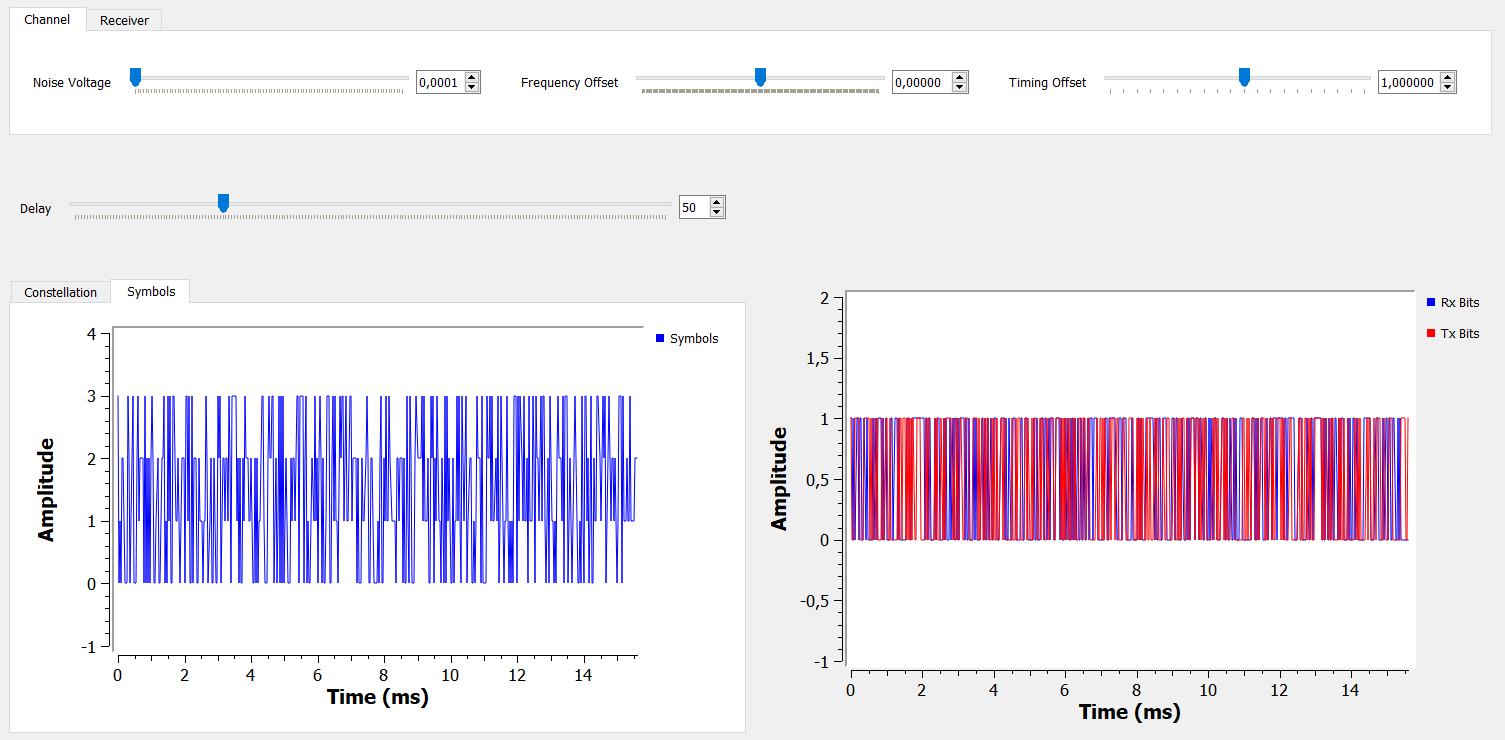
\includegraphics[width=0.8\textwidth]{fig7-2.PNG}
        \caption{Сравнение данных}
        \label{fig:fig7-2}
\end{figure}

\chapter{Выводы}
    В результате выполнения данной работы мы изучили остновные этапы, необходимые для восстановления сигналов, а также научились строить PSK модулятор/демодулятор для работы с сигналом.  
\end{document}